% StorePulse AI -- technical project report (IEEE conference format, IEEEtran).
% Build: see README.md in this folder (tectonic main.tex, or latexmk -pdf main.tex).
\documentclass[conference]{IEEEtran}

\usepackage{iftex}
\ifXeTeX
  \usepackage{fontspec}
  \setmainfont{texgyretermes}[Extension=.otf, UprightFont=*-regular, BoldFont=*-bold,
    ItalicFont=*-italic, BoldItalicFont=*-bolditalic]
\else
  \usepackage[T1]{fontenc}
  \usepackage[utf8]{inputenc}
  \usepackage{newtxtext}
\fi
\usepackage{cite}
\usepackage{amsmath,amssymb}
\usepackage{graphicx}
\usepackage{booktabs}
\usepackage{multirow}
\usepackage{array}
\usepackage[table]{xcolor}
\usepackage{tikz}
\usetikzlibrary{arrows.meta,positioning,shapes.geometric,shapes.misc,fit,calc,backgrounds}
\usepackage{listings}
\usepackage{xurl}
\usepackage[hidelinks=false,colorlinks=true,linkcolor=blue!55!black,citecolor=green!40!black,urlcolor=blue!60!black]{hyperref}
\usepackage[capitalise,nameinlink]{cleveref}
\usepackage{balance}

% ---------- Metadata ---------------------------------------------------------------------------------
\newcommand{\ProjectTitle}{StorePulse AI: A Multi-Tenant Platform for Leakage-Free Retail Demand Forecasting and Store-Level Operational Planning}
\newcommand{\AuthorName}{Bilal Shahid}
\newcommand{\Program}{Mathematics of Business and Industry}
\newcommand{\Supervisor}{Prof.\ Dr.\ Stefanie Vogl}
\newcommand{\University}{Ostbayerische Technische Hochschule Regensburg (OTH Regensburg)}
\newcommand{\Campus}{Regensburg, Germany}

\lstset{basicstyle=\ttfamily\scriptsize,breaklines=true,columns=fullflexible,frame=single,
  backgroundcolor=\color{gray!6},rulecolor=\color{gray!40}}
\newcommand{\code}[1]{\texttt{\small #1}}

\hypersetup{pdftitle={StorePulse AI -- Technical Project Report},pdfauthor={Bilal Shahid}}

\begin{document}

\title{\ProjectTitle}

\author{\IEEEauthorblockN{\AuthorName}
\IEEEauthorblockA{\Program\\
\University, \Campus\\
Supervisor: \Supervisor}}

\maketitle

\begin{abstract}
Store managers must decide every week how much stock to order and how many people to roster, yet
most small retailers plan from last year's sales and intuition. StorePulse AI is a multi-tenant web
platform that turns uploaded daily sales history into multi-horizon forecasts with P10--P90 ranges,
and then into a store-level operating plan: a profit-and-loss projection, a shift roster and a
ranked list of actions. The forecasting core trains gradient-boosted trees (LightGBM), feed-forward
and recurrent neural networks (MLP, GRU) and a weight-fitted ensemble on a shared, leakage-free
feature set, and compares them with seasonal-naive, ARIMA and SARIMA baselines. On all 1,115 stores
of the public Rossmann dataset, a rolling-origin backtest over eight 28-day windows, with no test data
used for model selection, shows LightGBM halving the weighted absolute percentage error (WAPE) of the
seasonal-naive benchmark at every origin (9.8 vs.\ 20.2\,\% on average; Diebold--Mariano $p<10^{-4}$).
On a common 30-day window the neural networks are significantly better than LightGBM (8.5 vs.\
9.7\,\%, $p<0.001$), whereas the ensemble's small advantage at 42 days (8.34 vs.\ 8.48\,\%) is not
significant ($p=0.063$). A shift-scheduling integer program, evaluated against realised footfall on
13,420 store-days, is not cheaper than the platform's rule-based plans at equal understaffing; its
value is to price the service level explicitly. Empirical P10--P90 bands cover 77--84\,\% of
hold-out days, and the interactive API answers in under 70\,ms. Limitations include one main data
set, consecutive backtest origins and an assumed hourly demand profile.
\end{abstract}

\begin{IEEEkeywords}
retail demand forecasting, gradient boosting, recurrent neural networks, forecast evaluation,
prediction intervals, workforce planning, multi-tenant SaaS, MLOps
\end{IEEEkeywords}

% =====================================================================================================
\section{Introduction}\label{sec:intro}

\subsection{Problem and motivation}
Daily demand drives almost every operating decision of a store: replenishment quantities, opening
hours, the number of staff on each shift and the expected profit of a promotion. Errors are
expensive in both directions---overstaffing wastes labour cost, understaffing loses sales and
service quality---and retail demand is shaped by weekly cycles, promotions, holidays and store
closures that simple rules of thumb capture poorly~\cite{fildes2022retail}. Forecasting competitions
have shown that machine-learning models, in particular gradient-boosted trees, now outperform
classical statistical methods on large retail data sets~\cite{makridakis2022m5}, but such models
rarely reach the person who plans next week's roster: they live in notebooks, require data-science
skills and stop at a number rather than a decision.

\subsection{Context and scope}
StorePulse AI is a software project developed in the repository \code{StorePulse\_AI} between
19 and 24 November 2026 (22 commits). It is a complete web application---FastAPI backend, Celery
workers, PostgreSQL, a Next.js user interface---plus a standalone command-line trainer that was
used on the GPU server of OTH Regensburg. The scope of this report is (i) the forecasting pipeline
and its evaluation, (ii) the conversion of forecasts into store plans (``Store Autopilot''), and
(iii) the engineering that makes both usable: multi-tenancy, background jobs, reproducible
training and an accessible user interface. Hosting a public production service is out of scope;
the platform runs locally or as a pilot.

\subsection{Contributions}
\begin{enumerate}
\item A leakage-free, direct multi-horizon feature pipeline in which every target-derived feature is
  lagged by $\lceil H/7\rceil\cdot 7$ days, verified by an automated scramble test (\cref{sec:features}).
\item A model zoo with a common interface---seasonal naive, ARIMA, SARIMA, LightGBM, MLP, GRU and a
  weight-fitted ensemble---evaluated on identical out-of-sample windows (\cref{sec:results-accuracy}).
\item A statistical evaluation: a rolling-origin backtest over eight 28-day origins with honest
  early stopping, Diebold--Mariano tests with a small-sample correction, and store-level bootstrap
  intervals (\cref{sec:math,sec:results-backtest,sec:results-significance}).
\item Empirical P10--P90 bands with a separate hold-out coverage check (\cref{sec:validation}).
\item A planning layer that converts forecasts into P\&L ranges, break-even revenue, shift
  headcounts and prioritised actions (\cref{sec:autopilot}), and a shift-scheduling integer program
  that is compared with the rule-based plan against realised footfall (\cref{sec:results-staffing}).
\item A reproducible engineering setup: a Docker-free local stack, GPU training on university
  hardware with checkpoint import, a 57-test suite, and measured performance figures
  (\cref{sec:results-system}).
\end{enumerate}

% =====================================================================================================
\section{Goals and Research Question}\label{sec:rq}

\subsection{Goals stated in the project materials}
The repository documentation (\code{CLAUDE.md}, \code{README.md}, \code{docs/}) states the following
goals, paraphrased here: G1---offer retail demand forecasting as a multi-tenant service in which
each organisation only sees its own stores, data and models; G2---go from an uploaded sales file to
schema mapping, data-health diagnostics, model training and tuning, multi-horizon and event
forecasts without writing code; G3---produce P\&L and workforce plans and a ``Store Autopilot''
with what-if scenarios and prescriptive actions; G4---compute everything from stored data and
configuration only (``no mock data in production paths''), raising a validation error when an input
is missing; G5---support GPU training and export reports as CSV, Excel and PDF.

\subsection{Research question formulated for this report}
The project materials do not state a research question. For this report the following question was
formulated so that each part can be answered with a statistical test or an optimisation result:

\begin{quote}\itshape
RQ: Under an evaluation protocol in which no test data influence model selection, does a global
gradient-boosted model forecast daily store sales significantly more accurately than the
seasonal-naive benchmark across forecast origins, and can the resulting probabilistic forecasts be
turned into staffing plans that cost less than the platform's rule-based plans without more
understaffing?
\end{quote}

\noindent It is split into three hypotheses:
\begin{itemize}
\item \textbf{H1 (accuracy over time):} Over $K=8$ rolling 28-day origins, LightGBM has lower WAPE
  than the seasonal-naive forecast. Tested with the Diebold--Mariano test (HLN correction) on the
  pooled daily loss differential and a sign test across origins (\cref{sec:results-backtest}).
\item \textbf{H2 (model differences):} On a common validation window, the differences between the
  learned models (ensemble, MLP, GRU, LightGBM) are statistically significant. Tested with the same
  DM test and a store-level bootstrap (\cref{sec:results-significance}).
\item \textbf{H3 (planning):} A cost-minimising integer program needs fewer paid staff-hours than the
  rule-based plan built from the same forecast, without increasing understaffing measured against
  realised footfall (\cref{sec:results-staffing}).
\end{itemize}
A secondary, engineering question asks whether forecasts and plans are fast and reproducible enough
for interactive use on commodity hardware (\cref{sec:results-system}).

% =====================================================================================================
\section{Literature Review and Related Work}\label{sec:related}

\subsection{Retail forecasting practice}
Fildes, Ma and Kolassa~\cite{fildes2022retail} review retail forecasting and stress that store-level
daily demand is driven by calendar effects, promotions and price, that hierarchies (store, category,
item) matter, and that forecasts are only valuable when connected to decisions such as
replenishment and staffing. StorePulse adopts this view by treating promotions, closures and
holidays as known-future covariates and by attaching planning outputs to every forecast.

\subsection{Statistical baselines}
Seasonal-naive forecasts and ARIMA-family models remain the standard reference points in
forecasting practice~\cite{hyndman2021fpp3}. They are cheap and interpretable, but are fitted per
series and do not share information across stores. StorePulse implements ARIMA(1,1,1) and a
SARIMA variant with a weekly seasonal term through \code{statsmodels}~\cite{seabold2010statsmodels,statsmodelssarimax},
and a weekday-aligned seasonal-naive model, so that every learned model can be compared with them.

\subsection{Machine learning and the M competitions}
The M4 competition found that hybrid and combined methods beat pure statistical
ones~\cite{makridakis2020m4}; its winner combined exponential smoothing with a recurrent
network~\cite{smyl2020hybrid}. In the retail-focused M5 competition, gradient-boosted trees
(LightGBM~\cite{ke2017lightgbm}) trained globally across many series dominated the
leaderboard~\cite{makridakis2022m5}. Global models learn shared patterns---such as the effect of a
promotion---from all series at once, which is why StorePulse trains one model across all stores of a
data set rather than one per store. Boosting libraries such as XGBoost~\cite{chen2016xgboost} and
LightGBM differ mainly in tree-growth strategy and speed; LightGBM was chosen for its histogram-based
training, native categorical handling, Tweedie and quantile objectives~\cite{lightgbmdocs}.

\subsection{Neural sequence models}
Recurrent networks such as LSTM~\cite{hochreiter1997lstm} and the lighter GRU~\cite{cho2014gru}
read a window of recent observations. Hewamalage et al.~\cite{hewamalage2021rnn} show that
recurrent networks are competitive when series are numerous and input pre-processing (scaling,
deseasonalisation) is done carefully, but rarely dominate tuned baselines on their own. Probabilistic
architectures such as DeepAR~\cite{salinas2020deepar} and the Temporal Fusion
Transformer~\cite{lim2021tft} forecast quantiles directly and combine static, known-future and
observed inputs---the same input taxonomy StorePulse uses. Implementing these architectures fully was
out of scope; the platform instead pairs a tabular MLP and a GRU encoder with the shared feature set,
implemented in PyTorch~\cite{paszke2019pytorch}.

\subsection{Forecast combination}
Combining forecasts often reduces error because individual models make partly independent
mistakes~\cite{bates1969combination}. StorePulse fits blend weights on the first half of the
validation window and reports the blend only on the untouched second half, avoiding the optimistic
bias of weights fitted on the evaluation data.

\subsection{Evaluation methodology}
Hyndman and Koehler~\cite{hyndman2006another} recommend scaled errors such as MASE because
percentage errors are undefined at zero and scale-dependent errors cannot be compared across series;
the M5 competition used the squared variant RMSSE~\cite{makridakis2022m5}. Tashman~\cite{tashman2000outofsample}
argues for strictly out-of-sample evaluation with a fixed origin or rolling origins; Bergmeir et
al.~\cite{bergmeir2018cv} discuss when cross-validation is valid for autoregressive models.
Uncertainty should be judged with proper scoring rules such as the pinball (quantile)
loss~\cite{gneiting2007proper,koenker1978quantiles}. StorePulse reports WAPE, RMSSE, RMSPE, R$^2$,
bias, interval coverage and pinball losses on a held-out window (\cref{sec:metrics}).

\subsection{Intermittent demand and staffing}
Item-level retail demand is often intermittent; Croston's method~\cite{croston1972intermittent}
separates the size of non-zero demand from the interval between sales, an idea StorePulse uses as
features (non-zero rate, mean non-zero size, days since last sale). Workforce planning is a large
operations-research field~\cite{ernst2004staff}; StorePulse deliberately uses a transparent
rule-based shift model (\cref{sec:autopilot}) rather than an optimiser, because its first goal is to
explain a plan to a store manager.

\subsection{Positioning}
Compared with competition solutions, which optimise a single leaderboard metric offline, and with
research architectures such as DeepAR or TFT, StorePulse focuses on the full path from raw upload to
an explainable plan, under multi-tenant security constraints (JWT authentication~\cite{rfc7519},
OWASP access-control guidance~\cite{owasp2021top10}) and with an accessible interface~\cite{w3c2023wcag22}.
Its novelty lies in the integration and in the evaluation discipline, not in a new model class.

% =====================================================================================================
\section{Methodology and System Design}\label{sec:design}

\subsection{Architecture}
\Cref{fig:architecture} shows the deployed components. The browser talks only to the Next.js
server~\cite{nextjsdocs}, which serves the UI and proxies \code{/api/v1} to the FastAPI
backend~\cite{fastapidocs}. All state lives in PostgreSQL~\cite{postgresdocs}; long-running work is
executed by Celery workers~\cite{celerydocs} on three queues (ingestion, training, forecasting).
Tasks receive only a row id, read all inputs from the database and write progress back through a
throttled reporter, so the UI can poll every two seconds and any task can be re-run idempotently.
Artifacts (raw uploads, canonical Parquet, model checkpoints, forecasts) are stored under
tenant-prefixed keys on local disk or S3-compatible storage.

\begin{figure}[t]
\centering
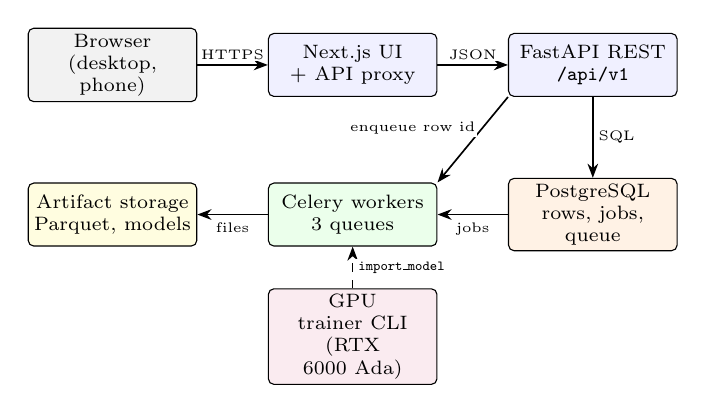
\begin{tikzpicture}[
  box/.style={draw, rounded corners=2pt, align=center, font=\scriptsize, text width=20mm,
              minimum height=8mm, inner sep=2pt, fill=#1},
  box/.default=blue!6,
  arr/.style={-{Stealth[length=1.8mm]}, semithick},
  lbl/.style={font=\tiny, fill=white, inner sep=0.8pt}]
\node[box=gray!10]    (browser) at (0,0)       {Browser\\(desktop, phone)};
\node[box]            (next)    at (3.05,0)    {Next.js UI\\+ API proxy};
\node[box]            (api)     at (6.1,0)     {FastAPI REST\\\texttt{/api/v1}};
\node[box=yellow!12]  (store)   at (0,-1.9)    {Artifact storage\\Parquet, models};
\node[box=green!8]    (workers) at (3.05,-1.9) {Celery workers\\3 queues};
\node[box=orange!10]  (db)      at (6.1,-1.9)  {PostgreSQL\\rows, jobs, queue};
\node[box=purple!8]   (gpu)     at (3.05,-3.45){GPU trainer CLI\\(RTX 6000 Ada)};
\draw[arr] (browser) -- node[lbl,above=1pt] {HTTPS} (next);
\draw[arr] (next) -- node[lbl,above=1pt] {JSON} (api);
\draw[arr] (api) -- node[lbl,right=1pt] {SQL} (db);
\draw[arr] (api.south west) -- node[lbl,pos=0.45,above left=-1pt] {enqueue row id} (workers.north east);
\draw[arr] (db) -- node[lbl,below=2pt] {jobs} (workers);
\draw[arr] (workers) -- node[lbl,below=2pt] {files} (store);
\draw[arr, dashed] (gpu) -- node[lbl,right=1pt] {\texttt{import\_model}} (workers);
\end{tikzpicture}
\caption{System architecture. Solid arrows: runtime requests; dashed: offline import of a model
trained on the university GPU. Every tenant-owned row and storage key carries the organisation id.}
\label{fig:architecture}
\end{figure}

\paragraph*{Multi-tenancy and security}
Every tenant table has an indexed \code{organization\_id}; services fetch rows only through a
helper that filters by the caller's organisation and returns 404 (not 403) for foreign rows, so the
existence of other tenants' data is not revealed. Roles (viewer, analyst, admin, owner) gate write
endpoints. Authentication uses short-lived JWT access tokens and refresh tokens~\cite{rfc7519};
storage keys are built from ids, never from user input. These choices map to the
``broken access control'' risk that leads the OWASP Top~10~\cite{owasp2021top10}.

\subsection{End-to-end workflow}
\Cref{fig:flow} shows the user flow with its decision points. A user uploads a CSV or Parquet file;
the backend profiles it and suggests a column mapping. After the mapping is confirmed, ingestion
streams the file into a canonical long table (\code{ds, store\_code, item\_id, y, \ldots}), applies
joins with auxiliary tables (e.g.\ M5 calendars and prices) and runs data-health diagnostics.
Models are trained or tuned on that table and appear on a leaderboard; any finished model can
forecast up to its trained horizon, and with a store's financial configuration the Autopilot turns
the forecast into a plan and exports.

\begin{figure}[t]
\centering
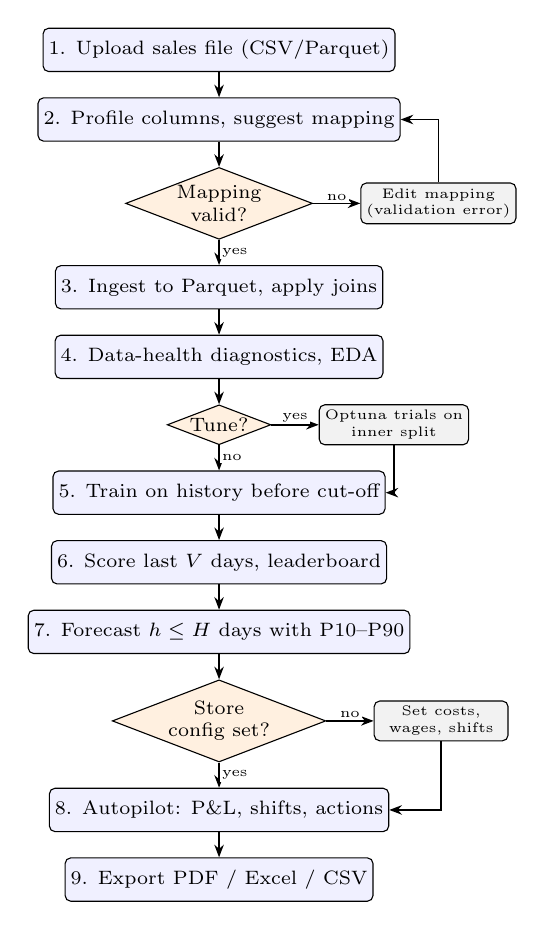
\begin{tikzpicture}[
  node distance=3.2mm,
  stp/.style={draw, rounded corners=2pt, fill=blue!6, font=\scriptsize, align=center,
               minimum width=36mm, minimum height=5.5mm, inner sep=2pt},
  dec/.style={draw, diamond, aspect=2.6, fill=orange!12, font=\scriptsize, align=center, inner sep=0.5pt},
  side/.style={draw, rounded corners=2pt, fill=gray!10, font=\tiny, align=center, minimum width=17mm, inner sep=2pt},
  arr/.style={-{Stealth[length=1.6mm]}, semithick},
  lab/.style={font=\tiny, fill=white, inner sep=0.8pt}]
\node[stp] (up) {1. Upload sales file (CSV/Parquet)};
\node[stp, below=of up] (prof) {2. Profile columns, suggest mapping};
\node[dec, below=of prof] (map) {Mapping\\valid?};
\node[side, right=6mm of map] (fix) {Edit mapping\\(validation error)};
\node[stp, below=of map] (ing) {3. Ingest to Parquet, apply joins};
\node[stp, below=of ing] (diag) {4. Data-health diagnostics, EDA};
\node[dec, below=of diag] (tune) {Tune?};
\node[side, right=6mm of tune] (opt) {Optuna trials on\\inner split};
\node[stp, below=of tune] (train) {5. Train on history before cut-off};
\node[stp, below=of train] (val) {6. Score last $V$ days, leaderboard};
\node[stp, below=of val] (fc) {7. Forecast $h \le H$ days with P10--P90};
\node[dec, below=of fc] (cfg) {Store\\config set?};
\node[side, right=6mm of cfg] (setcfg) {Set costs,\\wages, shifts};
\node[stp, below=of cfg] (auto) {8. Autopilot: P\&L, shifts, actions};
\node[stp, below=of auto] (exp) {9. Export PDF / Excel / CSV};
\draw[arr] (up) -- (prof);
\draw[arr] (prof) -- (map);
\draw[arr] (map) -- node[lab,above] {no} (fix);
\draw[arr] (fix.north) |- (prof.east);
\draw[arr] (map) -- node[lab,right] {yes} (ing);
\draw[arr] (ing) -- (diag);
\draw[arr] (diag) -- (tune);
\draw[arr] (tune) -- node[lab,above] {yes} (opt);
\draw[arr] (opt.south) |- (train.east);
\draw[arr] (tune) -- node[lab,right] {no} (train);
\draw[arr] (train) -- (val);
\draw[arr] (val) -- (fc);
\draw[arr] (fc) -- (cfg);
\draw[arr] (cfg) -- node[lab,above] {no} (setcfg);
\draw[arr] (setcfg.south) |- (auto.east);
\draw[arr] (cfg) -- node[lab,right] {yes} (auto);
\draw[arr] (auto) -- (exp);
\end{tikzpicture}
\caption{User and data flow from upload to plan. Diamonds are decisions; grey boxes are the side
paths a user takes when a decision is ``no'' or when tuning is requested.}
\label{fig:flow}
\end{figure}

\subsection{Leakage-free direct multi-horizon features}\label{sec:features}
A model trained for horizon $H$ must forecast every day $t+1,\ldots,t+H$ from information available
at the forecast origin $t$. StorePulse uses the \emph{direct} strategy: a single model predicts any
day up to $H$ ahead, and every feature computed from the target is shifted by
\begin{equation}
  \textstyle o = \lceil H/7 \rceil \cdot 7 \text{ days},
\end{equation}
so a 42-day model reads sales no later than 42 days before the predicted date, and the shift stays
weekday-aligned. The 50 features of the Rossmann LightGBM model fall into seven groups:
calendar terms; weekday-aligned lags ($o$, $o{+}7$, $o{+}14$, $o{+}21$, $o{+}49$ days) and
\code{lag\_364}; rolling means, standard deviation and zero share; intermittency statistics
inspired by Croston~\cite{croston1972intermittent}; promotion and closure streaks computed from
known-future flags; group aggregates (store type and assortment level) with the series' ratio to
them; and store metadata (competition distance and age, Promo2 status). A unit test scrambles all
targets after a cut-off and asserts that no target-derived feature with an earlier lag origin
changes---a guard against the most common silent error in forecasting pipelines.

\paragraph*{Closed-day rule}
Rossmann stores are closed on most Sundays and holidays. Closed days are removed from training and
every model returns exactly zero where \code{Open}=0, implemented once in the base class so that all
model families obey it.

\subsection{Model families}\label{sec:models}
All families implement one interface (\code{fit}, \code{predict}, \code{predict\_quantiles},
\code{save}/\code{load}).
\textbf{Seasonal naive} repeats the value of the same weekday of the last observed week.
\textbf{ARIMA(1,1,1)} and \textbf{SARIMA} (adding a weekly seasonal AR term) are fitted per series
with \code{statsmodels}; checkpoints store only the series and parameters and re-filter at forecast
time, which reduced a SARIMA checkpoint from about 16\,MB per series to under 100\,kB.
\textbf{LightGBM} uses 4,000 boosting rounds with early stopping (best iteration 445 at
$H{=}42$), 63 leaves and learning rate 0.05; the objective switches to Tweedie for zero-heavy
targets. The \textbf{MLP} feeds embeddings of categorical ids and signed-log-compressed numeric
features into hidden layers of 128 and 64 units, trained in $\log(1{+}y)$ space with optional
quantile heads. The \textbf{GRU} encodes the last 56 days of sales (scaled by the mean of open days)
plus open and promotion channels and fuses the result with the tabular path (best epoch 19 of 30).
The \textbf{ensemble} trains LightGBM and the GRU and blends them (\cref{sec:validation}).

\subsection{Validation, tuning and intervals}\label{sec:validation}
The last $V$ days of history (default $V=H$) are held out; all reported metrics come from that
window. Optuna~\cite{akiba2019optuna} trials are scored on an \emph{inner} split---the last $V$ days
of the training period---and the best configuration is then retrained with a fixed number of rounds
or epochs, so tuning never sees the reported window. Ensemble weights are fitted on the first half
of the validation window and all variants are compared on the second half. For models without
quantile heads, an empirical P10--P90 band is formed from the 10th and 90th percentiles of relative
validation residuals; its coverage is measured both in-sample and on a hold-out (calibrated on the
first half, measured on the second).

\paragraph*{Model selection inside the validation window} In the platform's default training path,
LightGBM's early stopping (patience 100 rounds) and the neural networks' best-epoch selection monitor
the loss on the validation window, i.e.\ the window on which the metrics are reported. This uses test
data for one scalar choice (the number of rounds or epochs). The single-split results in
\cref{tab:accuracy} were produced this way; the rolling-origin backtest (\cref{sec:results-backtest})
therefore uses an honest protocol in which the round count is chosen on the last $H$ days before the
test window and the model is then refitted on all training data.

\subsection{Mathematical formulation}\label{sec:math}
\paragraph*{Forecasting problem} Let $y_{i,t}\ge 0$ be the sales of store $i\in\{1,\dots,N\}$ on day
$t$, $\mathbf{z}_{i,t}$ the known-future covariates (open, promotion, holidays) and $\mathbf{s}_i$
static store attributes. At origin $T$ a single \emph{direct} model $f$ forecasts every lead time
$h=1,\dots,H$:
\begin{equation}
  \hat y_{i,T+h} = f\bigl(\mathbf{x}_{i,T+h}\bigr),\qquad
  \mathbf{x}_{i,t} = \bigl(\phi(y_{i,\le t-o}),\ \mathbf{z}_{i,t},\ \mathbf{s}_i,\ \text{calendar}(t)\bigr),
\end{equation}
where $\phi$ collects all target-derived features (lags, rolling statistics, group aggregates) and
$o$ is the lag offset.

\paragraph*{Leakage-freeness} With $o=\lceil H/7\rceil\cdot 7$ we have $o\ge H\ge h$, hence
$t-o = T+h-o \le T$: every target value used for any lead time is observed at the origin, so the same
model is valid for all $h\le H$ without recursion. Because $o\equiv 0 \pmod 7$, the most recent lag
$y_{i,t-o}$ falls on the same weekday as $t$, which preserves the strong weekly pattern of retail
sales. The price of this choice is that near lead times ($h\ll H$) cannot use the most recent
$o-h$ days.

\paragraph*{Training objective and closed days} Closed days ($\text{open}_{i,t}=0$) are removed from
training and forecast as exactly zero. LightGBM minimises the squared error $\sum (y-\hat y)^2$ (or a
Tweedie deviance for zero-heavy targets); the MLP and GRU minimise the squared error of the
standardised $\log(1+y)$.

\paragraph*{Ensemble weights} For two members with forecasts $\hat y^{(1)},\hat y^{(2)}$ the blend
is $\hat y^{(w)} = w\,\hat y^{(1)} + (1-w)\,\hat y^{(2)}$ with
\begin{equation}
  w^\ast = \arg\min_{w\in\{0,0.05,\dots,1\}} \mathrm{WAPE}\bigl(y,\hat y^{(w)}\bigr),
\end{equation}
computed on the first half of the validation window; every variant is scored on the second half only. The convex combination guarantees that the
blend's absolute error is never above the weighted average of the members' errors (triangle
inequality), which is why combining rarely hurts~\cite{bates1969combination}.

\paragraph*{Prediction band} For models without quantile heads, the relative residuals
$\rho = y/\hat y - 1$ on validation days with $y,\hat y>0$ give the empirical quantiles
$\hat q_{0.1},\hat q_{0.9}$, and the band is $[\hat y(1+\hat q_{0.1}),\ \hat y(1+\hat q_{0.9})]$.
It assumes that relative errors are exchangeable across stores and days; its hold-out coverage tests
that assumption.

\paragraph*{Diebold--Mariano test} For two forecasts $A,B$ of the same store-days define the daily
loss differential, scaled so that it sums to the WAPE difference,
\begin{equation}
  d_t = \frac{\sum_i \bigl(|y_{i,t}-\hat y^A_{i,t}| - |y_{i,t}-\hat y^B_{i,t}|\bigr)}
             {\sum_{i,s} y_{i,s}},\qquad \sum_t d_t = \mathrm{WAPE}_A - \mathrm{WAPE}_B .
\end{equation}
Aggregating over stores first keeps the common daily shocks (weather, holidays) that make store
errors correlated. Under $H_0: \mathbb{E}[d_t]=0$,
\begin{equation}
  \mathrm{DM} = \frac{\bar d}{\sqrt{\hat\sigma^2_{\mathrm{NW}}/T}},\qquad
  \hat\sigma^2_{\mathrm{NW}} = \hat\gamma_0 + 2\sum_{k=1}^{L}\Bigl(1-\tfrac{k}{L+1}\Bigr)\hat\gamma_k ,
\end{equation}
with the Newey--West long-run variance~\cite{newey1987hac} and lag $L=\lfloor 4(T/100)^{2/9}\rfloor$
\cite{diebold1995comparing}. Because $T$ is small (28--224 days), the statistic is multiplied by the
Harvey--Leybourne--Newbold factor $\sqrt{(T+1-2h+h(h-1)/T)/T}$ with $h=L+1$ and compared with a
Student-$t_{T-1}$ distribution~\cite{harvey1997testing}.

\paragraph*{Store bootstrap} As a complementary measure, stores are resampled with replacement
($B=2000$) and $\mathrm{WAPE}_A-\mathrm{WAPE}_B$ is recomputed on each resample; the 2.5 and 97.5\,\%
percentiles form a 95\,\% interval. Resampling whole stores keeps each store's days together (a
block bootstrap with the store as block~\cite{kunsch1989jackknife}). It answers ``would the difference
hold for a different set of stores?'', whereas DM answers ``would it hold on other days?''. The two can
disagree when errors share common daily shocks.

\paragraph*{Staffing integer program} For one store-day with forecast footfall $F$, let $p_t$ be the
share of customers in hour $t=0,\dots,11$, $c$ the customers one employee serves per hour and $m$ the
minimum staff on the floor. The hourly requirement is
\begin{equation}
  r_t = \max\bigl(m,\ \lceil F p_t / c\rceil\bigr).
\end{equation}
Shift templates $j=(s_j,\ell_j)$ start at hour $s_j$ and last $\ell_j\in\{4,6,8\}$ hours; $a_{tj}=1$
if template $j$ covers hour $t$. With $x_j\in\mathbb{Z}_{\ge0}$ workers on template $j$, the
set-covering formulation of Dantzig~\cite{dantzig1954comment} is
\begin{equation}
  \min_{x\in\mathbb{Z}^{J}_{\ge 0}} \ \sum_j \ell_j x_j
  \quad\text{s.t.}\quad \sum_j a_{tj} x_j \ \ge\ r_t,\ \ t=0,\dots,11 .
\end{equation}
The objective is paid staff-hours (labour cost is the hourly wage times this value). A service-level
variant plans on the P90 forecast, $F_{0.9}=\hat y(1+\hat q_{0.9})/\bar b_i$, where $\bar b_i$ is the
store's average basket (sales per customer). Plans are evaluated against the requirement implied by
the \emph{realised} footfall, with understaffing $\sum_t \max(0, r^{\text{act}}_t - \text{staff}_t)$.

\subsection{Store Autopilot}\label{sec:autopilot}
The Autopilot is a pure function from (model, data, store configuration, scenario) to a JSON plan.
For a window (next day, 7 or 30 days, or a custom range within the model horizon) it forecasts
revenue P10/P50/P90; converts sales to footfall using the customers column, a historical basket size
or a configured average transaction value; and computes cost of goods, gross profit, labour (planned
on P50), fixed overhead, net profit for each band, break-even revenue
\begin{equation}
  R_{\text{BE}} = \frac{\text{labour} + \text{overhead}}{\text{contribution ratio}},
\end{equation}
and margin of safety. Footfall is split into shifts (default 30/45/25\,\% for morning, midday peak
and evening); each shift receives $\max(\text{min staff}, \lceil \text{required hours}/\text{shift
hours}\rceil)$ people, capped by a maximum, and peak-hour gaps are covered by floaters. Actions are
ranked by severity and money at stake: loss days, downside below break-even, capacity limits, idle
labour, closures, holidays, promotion profitability against a baseline plan, anomalies and model
uncertainty. Scenario levers (promotion, holidays, demand shocks, price changes with elasticity,
cost overrides) re-forecast through the model and are diffed against the baseline. Every default is
echoed in an \code{assumptions} section, because planning conventions are not data.

\subsection{User interface}
The Next.js interface has eight authenticated pages (\cref{fig:screens}). It uses TanStack Query for
server state with two-second polling while jobs run. A redesign during the project introduced a
token-based dark ``storm'' theme whose text colours were checked against WCAG~2.2 contrast
requirements~\cite{w3c2023wcag22} (\cref{tab:contrast} in the appendix), visible keyboard focus and
reduced-motion support. For presentations without hosting costs, the local stack can expose the UI
through a free Cloudflare quick tunnel~\cite{cloudflaretunnel}.

\subsection{Evaluation procedure}\label{sec:procedure}
\textbf{Data.} The main evaluation uses the public Rossmann Store Sales data~\cite{kaggle2015rossmann}
(1,017,209 store-days, 1,115 stores, 1 Jan 2013--31 Jul 2015) with store metadata. A second data set,
the Corporaci\'on Favorita store sales~\cite{kaggle2021storesales} (3,000,888 rows, 54 stores $\times$
33 product families, 2013--2017), and a three-store synthetic data set exercise product rankings and
edge cases. \textbf{Split.} For horizon $H\in\{30,42\}$ the last $H$ days are held out
(42 days: 20 Jun--31 Jul 2015, 46,830 store-days; 30 days: 2 Jul--31 Jul 2015, 33,450 store-days);
every model of the same horizon is scored on the same rows. \textbf{Backtest.} Eight rolling
origins with consecutive 28-day test windows (20 Dec 2014--31 Jul 2015, 242,560 store-days) compare
LightGBM and the seasonal-naive model; for each origin the data are truncated at the end of the test
window and the whole pipeline is rerun. \textbf{Staffing.} Plans for 18--31 July 2015 are built from the
42-day ensemble forecast and evaluated against actual customer counts. \textbf{Environments.} Neural networks
and the ensembles were trained with the standalone CLI on the OTH JupyterHub host (NVIDIA RTX 6000
Ada, CUDA 12.6, PyTorch 2.14, LightGBM 4.7 with 16 threads); baselines and reproduction runs used a
laptop (Intel Core i7-8665U, 4 cores, 24\,GB RAM, no CUDA GPU). \textbf{System measurements.} API
latency was measured on the laptop with 30 sequential calls per endpoint after one warm-up call;
job durations come from the start and finish timestamps the workers record. Commands are listed in
\cref{app:repro}.

% =====================================================================================================
\section{Evaluation Metrics}\label{sec:metrics}
Let $y_i$ be actual and $\hat y_i$ forecast daily sales (in euros for Rossmann) over the $n$
store-days of the validation window.

\begin{itemize}
\item \textbf{WAPE} (\%) $=\sum_i |y_i-\hat y_i| / \sum_i |y_i|$. It is defined when individual days
  are zero (closed stores), weights large stores by their sales, and reads as ``euros of error per
  euro sold''. \textbf{Accuracy} $=1-\text{WAPE}$ is shown in the UI. Primary metric.
\item \textbf{RMSE} and \textbf{MAE} (EUR per store-day): scale-dependent absolute errors.
\item \textbf{RMSPE} (unitless): root mean squared percentage error over days with $y_i>0$, the
  official Rossmann competition metric~\cite{kaggle2015rossmann}.
\item \textbf{RMSSE} (unitless): per-series RMSE divided by the in-sample RMSE of the one-step
  naive forecast, averaged over series, as in M5~\cite{makridakis2022m5,hyndman2006another}. Values
  below 1 beat a naive forecast's typical one-step error.
\item \textbf{R$^2$}: share of variance explained. \textbf{Bias} (\%) $=\sum(\hat y-y)/\sum y$:
  positive values over-forecast.
\item \textbf{Interval coverage} (\%): share of days inside $[\hat y_{10}, \hat y_{90}]$; nominal 80\,\%.
  We report the \emph{hold-out} coverage, because in-sample coverage is inflated by closed days that
  are always covered (identical 82.8\,\% for every model at 42 days).
\item \textbf{DM statistic and $p$-value}, \textbf{95\,\% bootstrap interval} (percentage points of
  WAPE) and a \textbf{sign test} over origins: significance of accuracy differences (\cref{sec:math}).
\item \textbf{Paid staff-hours} and \textbf{understaffing} (staff-hours below the requirement implied
  by realised footfall): cost and service of a staffing plan.
\item \textbf{Training time} (s), \textbf{job duration} (s) and \textbf{API latency} (ms, median and
  95th percentile): operational cost and responsiveness.
\end{itemize}
The seasonal-naive forecast is the baseline for H1; ARIMA and SARIMA are the classical statistical
references; the rule-based plan is the baseline for H3.

% =====================================================================================================
\section{Results}\label{sec:results}

\subsection{Forecast accuracy}\label{sec:results-accuracy}
\Cref{tab:accuracy} and \cref{fig:accuracy} compare all models on identical windows. At 42 days the
weight-fitted ensemble is best (WAPE 8.34\,\%), followed by LightGBM (8.48\,\%); every
machine-learning model more than halves the error of the seasonal-naive baseline (19.69\,\%) and of
ARIMA/SARIMA (21.86--22.56\,\%). At 30 days the GRU (8.52\,\%) and MLP (8.55\,\%) beat LightGBM
(9.70\,\%); the ensemble's weight search assigned the GRU a weight of 1.0, so its scores equal the
GRU's. ARIMA and SARIMA are worse than the seasonal-naive baseline in WAPE at both horizons---they
do not see promotions, which lift mean store sales by 38.8\,\% in this data set (\cref{fig:eda}).

\begin{table*}[t]
\centering
\caption{Out-of-sample accuracy on all 1,115 Rossmann stores. Lower is better except $R^2$. Best value per
horizon in bold. Sources: GPU host runs (\code{outputs/}); seasonal naive and 42-day ARIMA/SARIMA on the laptop
(same data, stores and window); ``--'' = not recorded for that run.}
\label{tab:accuracy}
\scriptsize
\begin{tabular}{@{}llrrrrrrrr@{}}
\toprule
Horizon & Model & WAPE (\%) & RMSE (EUR) & MAE (EUR) & RMSPE & RMSSE & $R^2$ & Bias (\%) & Fit (s) \\
\midrule
\multirow{7}{*}{42 days} & Seasonal naive & 19.69 & 1,682.6 & 1,181.8 & 0.248 & 0.366 & 0.796 & $-2.78$ & 0.0 \\
 & ARIMA(1,1,1) & 22.56 & -- & -- & -- & 0.451 & -- & -- & 727.0 \\
 & SARIMA & 21.86 & -- & -- & -- & 0.416 & -- & -- & 1,694.5 \\
 & LightGBM & 8.48 & 803.3 & 508.9 & 0.124 & 0.164 & 0.954 & $+1.68$ & 11.2 \\
 & MLP & 8.72 & 831.4 & 523.4 & \textbf{0.124} & 0.170 & 0.950 & $\mathbf{-0.50}$ & 10.8 \\
 & GRU & 8.86 & 845.1 & 531.7 & 0.126 & 0.172 & 0.949 & $-0.07$ & 43.3 \\
 & Ensemble (0.75 LGBM + 0.25 GRU) & \textbf{8.34} & \textbf{793.3} & \textbf{500.8} & 0.122 & \textbf{0.162} & \textbf{0.955} & $+1.22$ & 43.9 \\
\midrule
\multirow{6}{*}{30 days} & Seasonal naive & 19.54 & 1,646.5 & 1,187.5 & 0.251 & 0.359 & 0.792 & $-3.38$ & 0.0 \\
 & ARIMA(1,1,1) & 21.90 & 1,919.3 & 1,331.1 & 0.274 & 0.419 & 0.717 & $-16.09$ & 113.6 \\
 & SARIMA & 20.62 & 1,780.3 & 1,253.7 & 0.281 & 0.386 & 0.757 & $-7.14$ & 275.4 \\
 & LightGBM & 9.70 & 869.6 & 589.7 & 0.154 & 0.186 & 0.942 & $+0.55$ & 4.2 \\
 & MLP & 8.55 & \textbf{779.1} & 519.5 & 0.123 & \textbf{0.163} & \textbf{0.953} & $\mathbf{+0.12}$ & 114.1 \\
 & GRU (= ensemble, weight 1.0) & \textbf{8.52} & 789.4 & \textbf{517.9} & \textbf{0.121} & 0.163 & 0.952 & $-1.04$ & 227.3 \\
\bottomrule
\end{tabular}
\end{table*}

\begin{figure}[t]
\centering
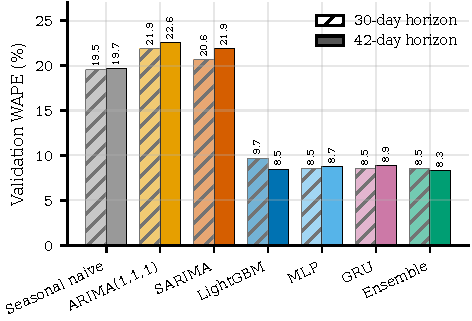
\includegraphics[width=\columnwidth]{figures/fig_accuracy.pdf}
\caption{Validation WAPE by model and horizon (bar labels in \%). Hatched bars: 30-day models.
Machine-learning models (right) roughly halve the error of the baselines (left).
Data: \code{data/fig\_accuracy\_source.csv}.}
\label{fig:accuracy}
\end{figure}

\paragraph*{Error by lead time and weekday}
\Cref{fig:weekahead} breaks the error down by week ahead. Error does not grow monotonically with
lead time: for the 42-day LightGBM model the first week is the easiest (6.96\,\%) and weeks~2--3 the
hardest (9.89 and 9.63\,\%); the cause was not isolated, and calendar effects inside the
window (e.g.\ school holidays) are one candidate explanation. Because all target features are lagged by the full offset, the first and the
last week ahead use the same information, so differences reflect the calendar rather than lead
time. By weekday (\cref{fig:weekday}) LightGBM is the most even model; the neural networks are
weakest on the few Sunday openings (12.0--12.4\,\% WAPE, strong negative bias), a rare
regime they see little of in training.

\begin{figure}[t]
\centering
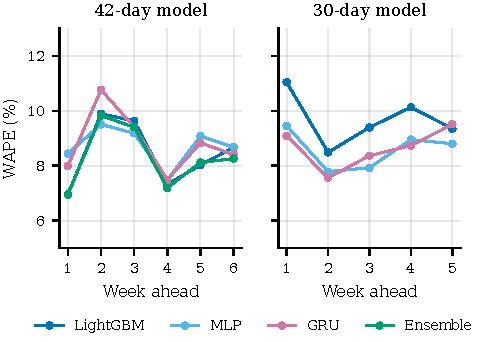
\includegraphics[width=\columnwidth]{figures/fig_week_ahead.pdf}
\caption{WAPE by week ahead within the validation window for the 42-day (left) and 30-day (right)
models; the 30-day ensemble equals the GRU and is not drawn. Baselines (19--32\,\%) are omitted so
the learned models remain distinguishable. Week 5 of the 30-day window contains only two days. Data:
\code{data/residuals\_by\_week\_ahead.csv}.}
\label{fig:weekahead}
\end{figure}

\begin{figure}[t]
\centering
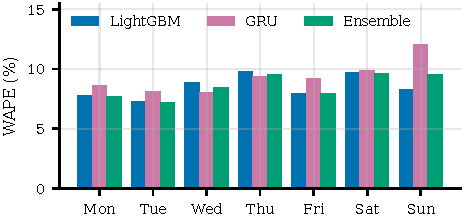
\includegraphics[width=\columnwidth]{figures/fig_weekday.pdf}
\caption{WAPE by weekday, 42-day models. Sunday WAPE covers only the stores that open on Sundays.
Data: \code{data/residuals\_by\_weekday.csv}.}
\label{fig:weekday}
\end{figure}

\paragraph*{Ensemble on untouched data}
\Cref{fig:ensemble} shows the 42-day comparison on the second half of the validation window
(23,415 store-days), which played no role in fitting the weights. The fitted blend (7.84\,\%)
improves on its members (LightGBM 8.01\,\%, GRU 8.34\,\%) and matches the equal-weight blend
(7.84\,\%), consistent with the forecast-combination literature~\cite{bates1969combination}.

\begin{figure}[t]
\centering
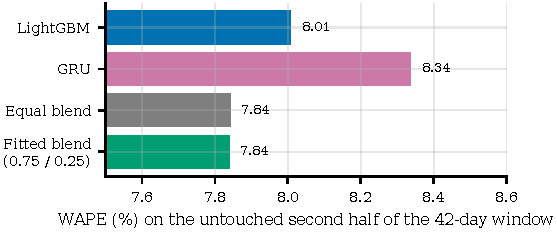
\includegraphics[width=\columnwidth]{figures/fig_ensemble.pdf}
\caption{42-day ensemble evaluated only on the second half of the validation window. Data:
\code{data/ensemble\_holdout.csv}.}
\label{fig:ensemble}
\end{figure}

\paragraph*{Documented ablations}
\Cref{tab:ablation} lists ablations recorded in the project log during development (42-day horizon,
same window). They were not re-run for this report and are reported as documented.

\begin{table}[t]
\centering
\caption{Ablations recorded in the project documentation (\code{CLAUDE.md}); not re-measured for this report.}
\label{tab:ablation}
\scriptsize
\begin{tabular}{@{}lr@{}}
\toprule
Variant (42-day, all stores) & Accuracy (\%) \\
\midrule
LightGBM, default parameters & 91.52 \\
LightGBM, 25-trial honest Optuna tuning & 91.77 \\
LightGBM, $\log(1{+}y)$ target & 91.36 \\
LightGBM, L1 objective & 91.29 \\
MLP without log-compressed inputs & 90.94 \\
MLP, 6-trial honest tuning (inner split 92.07) & 91.17 \\
MLP with quantile heads (band coverage 78.6\,\%) & 91.40 \\
\bottomrule
\end{tabular}
\end{table}

\paragraph*{Second data set}
On Favorita (54 stores $\times$ 33 product families, last two years of history, 28-day horizon),
LightGBM reaches a validation WAPE of 13.07\,\% (17 Jul--15 Aug 2017). The higher error is expected
for category-level series with many zero days, and the run demonstrates the product ranking shown in
\cref{fig:screens}d.

\subsection{Uncertainty}\label{sec:results-uncertainty}
\Cref{fig:coverage} shows the hold-out coverage of the P10--P90 bands. At 42 days all
machine-learning models cover 82.4--83.8\,\% of hold-out days, slightly above the nominal 80\,\%
(conservative). At 30 days LightGBM and the MLP stay close to nominal (81.5 and 82.8\,\%), while the
GRU falls to 77.2\,\% and ARIMA/SARIMA to 77.1 and 74.2\,\%, i.e.\ their bands are too narrow out of
sample. The seasonal-naive band covers 75.4\,\% (42 days) and 83.5\,\% (30 days), so its
calibration is unstable across windows. All baseline bands are more than twice as wide (mean width
about 3,500--4,300 EUR versus 1,580--1,920 EUR), i.e.\ much less sharp.

\begin{figure}[t]
\centering
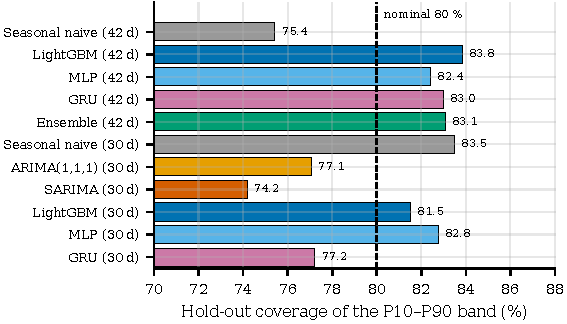
\includegraphics[width=\columnwidth]{figures/fig_coverage.pdf}
\caption{Hold-out coverage of the empirical P10--P90 band (calibrated on the first half of the
validation window, measured on the second). Dashed line: nominal 80\,\%. Data:
\code{data/interval\_coverage.csv}.}
\label{fig:coverage}
\end{figure}

\subsection{Rolling-origin backtest}\label{sec:results-backtest}
\Cref{fig:backtest} and \cref{tab:backtest} show LightGBM with honest early stopping against the
seasonal-naive model over eight consecutive 28-day test windows. LightGBM is better at \emph{every}
origin. Its WAPE ranges from 8.03 to 14.67\,\% (mean 9.82\,\%, 95\,\% $t$-interval over origins
7.93--11.71\,\%), against 16.22--31.10\,\% for the baseline (mean 20.19\,\%). Pooled over all 242,560
store-days the WAPE difference is $-10.32$ percentage points; the DM test over the 224 days gives
DM$^\ast=-10.90$ ($p<10^{-4}$), the sign test over origins $p=0.008$ (8 of 8), and the store
bootstrap $[-10.49,-10.14]$. H1 is supported.

Accuracy varies strongly over time. The Christmas window (20 Dec--16 Jan, only 935 stores because 180
stores lack data for late 2014) and the following window are the hardest for both models; summer
windows are the easiest. The single-split 42-day WAPE (8.48\,\%) is therefore at the favourable end of
what the model achieves across the year, and 9.8\,\% is the more representative figure.

Choosing the round count on the test window instead of the inner window made no systematic
difference: pooled WAPE 9.69 vs.\ 9.67\,\%, DM $p=0.92$, better in only 2 of 8 origins. The selected
round counts, however, are unstable under both protocols (45--1,273 with test-window stopping,
66--3,050 honestly), which shows that early stopping on a squared-error loss is a weak selector for a
WAPE-oriented model. The single-split LightGBM results in \cref{tab:accuracy} are thus unlikely to be
materially optimistic, although this was verified only for LightGBM.

\begin{figure}[t]
\centering
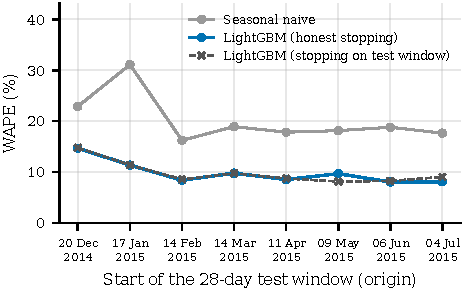
\includegraphics[width=\columnwidth]{figures/fig_backtest.pdf}
\caption{WAPE per rolling origin (28-day test windows, all stores). LightGBM with honest early stopping
beats the seasonal-naive model at every origin; stopping on the test window (dashed) makes no
systematic difference. Data: \code{data/backtest\_per\_origin.csv}.}
\label{fig:backtest}
\end{figure}

\begin{table}[t]
\centering
\caption{Rolling-origin backtest, eight 28-day origins (WAPE in \%). The interval is a Student-$t$
interval over origins; origins share training data, so it is approximate.}
\label{tab:backtest}
\scriptsize
\setlength{\tabcolsep}{3pt}
\begin{tabular}{@{}lrrrr@{}}
\toprule
Model & Mean & 95\,\% interval & Min & Max \\
\midrule
Seasonal naive & 20.19 & 16.16--24.21 & 16.22 & 31.10 \\
LightGBM, honest stopping & \textbf{9.82} & 7.93--11.71 & 8.03 & 14.67 \\
LightGBM, stopping on test window & 9.83 & 7.94--11.72 & 8.13 & 14.78 \\
\bottomrule
\end{tabular}
\end{table}

\subsection{Significance of model differences}\label{sec:results-significance}
\Cref{tab:dm} tests the differences of \cref{tab:accuracy} with the DM test (HLN correction,
Newey--West lag 3) and the store bootstrap of \cref{sec:math}. At 30 days the neural networks beat
LightGBM clearly ($p<0.001$, WAPE $-1.2$ percentage points) and LightGBM beats SARIMA ($p<0.001$),
whereas GRU and MLP are indistinguishable ($p=0.92$) and so are SARIMA and ARIMA ($p=0.69$). At 42
days the ensemble's 0.14-point advantage over LightGBM is \emph{not} significant at the 5\,\% level
over days ($p=0.063$), and neither are the MLP's and GRU's disadvantages ($p=0.49$, $0.10$).

The store bootstrap intervals for these 42-day pairs exclude zero. The two procedures answer
different questions: the bootstrap holds the 42 days fixed and asks whether the gap would persist
for another set of stores, while DM asks whether it would persist on other days. Because all stores
share daily shocks (weather, holidays, promotions), 42 days provide only about 42 independent pieces
of evidence, and on that basis the small 42-day differences are not established. These single-split
forecasts also selected their round or epoch count on the same window (\cref{sec:validation}).

\begin{table}[t]
\centering
\caption{Diebold--Mariano tests (HLN-corrected, two-sided) and 95\,\% store-bootstrap intervals for the
WAPE difference $A-B$ (percentage points). Negative values favour $A$.}
\label{tab:dm}
\scriptsize
\setlength{\tabcolsep}{3pt}
\begin{tabular}{@{}llrrrr@{}}
\toprule
$H$ & $A$ vs.\ $B$ & $\Delta$WAPE & DM$^\ast$ & $p$ & Bootstrap 95\,\% \\
\midrule
42 & Ensemble vs.\ LightGBM & $-0.14$ & $-1.91$ & 0.063 & $[-0.16, -0.11]$ \\
42 & MLP vs.\ LightGBM & $+0.24$ & $0.70$ & 0.489 & $[+0.16, +0.32]$ \\
42 & GRU vs.\ LightGBM & $+0.38$ & $1.69$ & 0.098 & $[+0.29, +0.47]$ \\
\midrule
30 & GRU vs.\ LightGBM & $-1.18$ & $-4.98$ & $<$0.001 & $[-1.31, -1.06]$ \\
30 & MLP vs.\ LightGBM & $-1.15$ & $-4.40$ & $<$0.001 & $[-1.29, -1.02]$ \\
30 & GRU vs.\ MLP & $-0.03$ & $-0.10$ & 0.920 & $[-0.11, +0.05]$ \\
30 & LightGBM vs.\ SARIMA & $-10.92$ & $-4.10$ & $<$0.001 & $[-11.32, -10.56]$ \\
30 & SARIMA vs.\ ARIMA & $-1.27$ & $-0.40$ & 0.694 & $[-1.57, -0.94]$ \\
\bottomrule
\end{tabular}
\end{table}

\subsection{Staffing: integer program versus rules}\label{sec:results-staffing}
The plans were built from the 42-day ensemble forecast for the last 14 days of its validation window
(18--31 July 2015, 13,420 open store-days) and judged against the hourly requirement implied by the
\emph{actual} customer counts (\cref{sec:math}; demo configuration: 20 customers per staff-hour,
at least two staff, 12 opening hours). The P50 integer program pays 1.5\,\% fewer staff-hours than the
rule plan but leaves 16\,\% more understaffing (22,233 vs.\ 19,121 staff-hours), because the rules'
rounding per four-hour block acts as an implicit buffer. Planning the integer program on the P90
forecast costs 8.1\,\% more hours and cuts understaffing by 65\,\% (\cref{tab:staffing}).

\Cref{fig:staffing} gives the fair comparison: scaling the planned footfall by a safety factor
$\lambda$ traces the optimiser's cost--understaffing frontier, and the rule plan lies \emph{on} it.
At the rule plan's understaffing the optimiser needs 605,711 paid hours versus the rules' 605,682
(interpolated, $+0.00\,\%$). H3 is therefore not supported in this setting: with three fixed shifts that
already match the assumed demand profile, a minimum of two staff and integer rounding, the simple rules
are cost-efficient. The value of the optimisation model lies elsewhere: it makes the trade-off
explicit, so a manager can choose a service level (for example $\lambda=1.06$: $+3.4\,\%$ hours,
$-32\,\%$ understaffing) instead of inheriting the one implied by rounding.

\begin{table}[t]
\centering
\caption{Staffing plans for 13,420 open store-days, evaluated against realised footfall.}
\label{tab:staffing}
\scriptsize
\setlength{\tabcolsep}{3pt}
\begin{tabular}{@{}lrrrr@{}}
\toprule
Plan & Paid hours & vs.\ rules & Understaffing & Days w/o gap \\
 & & (\%) & (staff-h) & (\%) \\
\midrule
Rules, P50 forecast & 605,682 & 0.0 & 19,121 & 67.5 \\
Integer program, P50 & 596,724 & $-1.5$ & 22,233 & 65.3 \\
Integer program, P90 & 655,026 & $+8.1$ & 6,705 & 87.3 \\
\bottomrule
\end{tabular}
\end{table}

\begin{figure}[t]
\centering
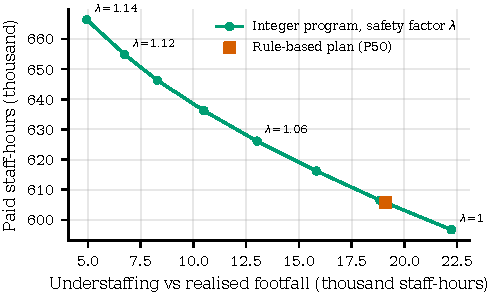
\includegraphics[width=\columnwidth]{figures/fig_staffing.pdf}
\caption{Cost--understaffing frontier of the integer program as the planned footfall is scaled by
$\lambda$ (1 = P50, 1.117 = P90), and the rule-based plan (square). Data:
\code{data/staffing\_frontier.csv}.}
\label{fig:staffing}
\end{figure}

\subsection{System performance and reproducibility}\label{sec:results-system}
\paragraph*{Reproducibility} Re-running LightGBM with the same code on the laptop CPU reproduced the
GPU host's validation WAPE to four decimal places at both horizons (0.08478 and 0.09700), at 48\,s
and 22\,s training time instead of 11.2\,s and 4.2\,s. Neural networks are not bit-reproducible
across devices: the 42-day MLP trained on the laptop CPU reached 8.46\,\% WAPE in 613.8\,s,
versus 8.72\,\% in 10.8\,s on the GPU (different batch size and floating-point order), a speed-up of
about 57$\times$ (\cref{fig:fittime}).

\begin{figure}[t]
\centering
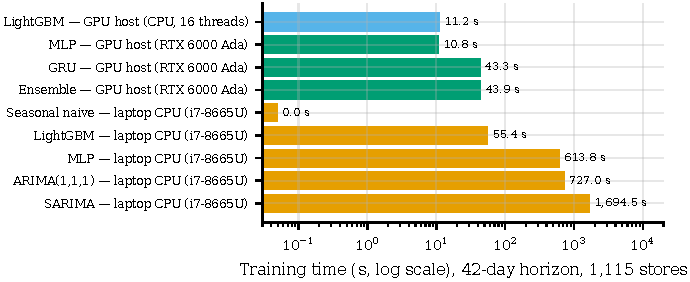
\includegraphics[width=\columnwidth]{figures/fig_fit_time.pdf}
\caption{Training time for a 42-day model on all 1,115 stores by model and machine (log scale).
Laptop values are the runs recorded by the application's Model Lab (LightGBM 55.4\,s there versus
48\,s in the database-free pipeline runner). Data: \code{data/fig\_fit\_time\_source.csv}.}
\label{fig:fittime}
\end{figure}

\paragraph*{Interactive latency} \Cref{tab:latency} and \cref{fig:latency} report API latency on
the laptop. Endpoints that drive the main pages---lists, the forecast series, P\&L and
workforce---answer in 3--54\,ms (median) and at most 70.5\,ms. The exploratory data analysis over
the full 1.0-million-row table takes 1.74\,s (median), acceptable for a page opened once per data set
but the slowest endpoint measured.

\begin{table}[t]
\centering
\caption{API latency on the laptop (loopback, one client, 30 sequential calls after one warm-up).}
\label{tab:latency}
\scriptsize
\begin{tabular}{@{}lrrr@{}}
\toprule
Endpoint & Median (ms) & P95 (ms) & Size (kB) \\
\midrule
\code{/health/ready} & 3.3 & 4.7 & 0.1 \\
\code{/model-runs} & 7.5 & 9.0 & 35.3 \\
\code{/stores} (50 rows) & 9.9 & 12.3 & 25.2 \\
\code{/forecasts/\{id\}/series} & 17.8 & 21.4 & 5.6 \\
\code{/forecasts/\{id\}/pnl} & 51.0 & 67.2 & 8.0 \\
\code{/forecasts/\{id\}/workforce} & 53.7 & 63.4 & 6.3 \\
\code{/datasets/\{id\}/eda} (1.0\,M rows) & 1,743.5 & 1,952.2 & 8.9 \\
\bottomrule
\end{tabular}
\end{table}

\begin{figure}[t]
\centering
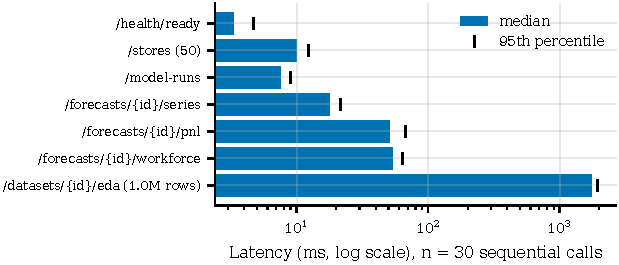
\includegraphics[width=\columnwidth]{figures/fig_latency.pdf}
\caption{API latency per endpoint (bars: median; ticks: 95th percentile; log scale). Data:
\code{data/api\_latency.csv}, raw calls in \code{data/api\_latency\_raw.csv}.}
\label{fig:latency}
\end{figure}

\paragraph*{Background jobs} Measured from worker timestamps on the laptop, a forecast over all
1,115 Rossmann stores took 9.3\,s median (5.0--38.1\,s, $n{=}7$) and an Autopilot plan for one
store 4.8\,s median (0.4--21.3\,s, $n{=}8$); on Favorita a forecast took 11.3--12.4\,s ($n{=}2$).
The longest runs include cold model loading after a worker start.

\paragraph*{Automated tests} The backend suite of 57 tests (API envelope and authentication,
finance arithmetic, Autopilot, joins and features including the leakage test, model round-trips,
EDA, local tooling and an end-to-end Rossmann pipeline) passed in 38.5\,s; the frontend passes the
TypeScript check and a production build (\cref{app:tests}).

\begin{figure*}[t]
\centering
\setlength{\tabcolsep}{2pt}
\begin{tabular}{cc}
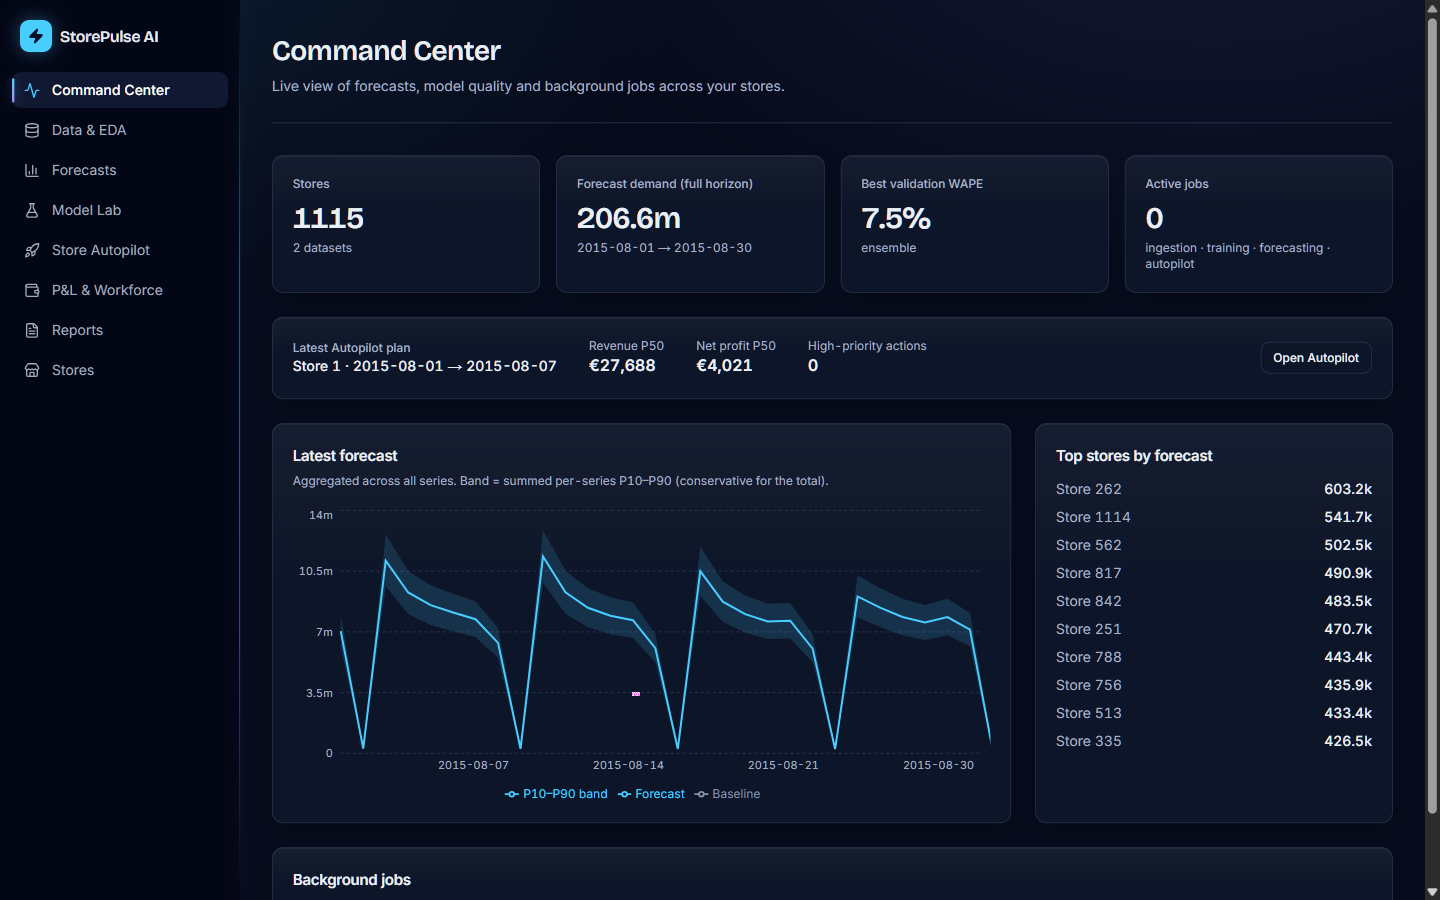
\includegraphics[width=0.49\textwidth]{figures/screens/command_center.png} &
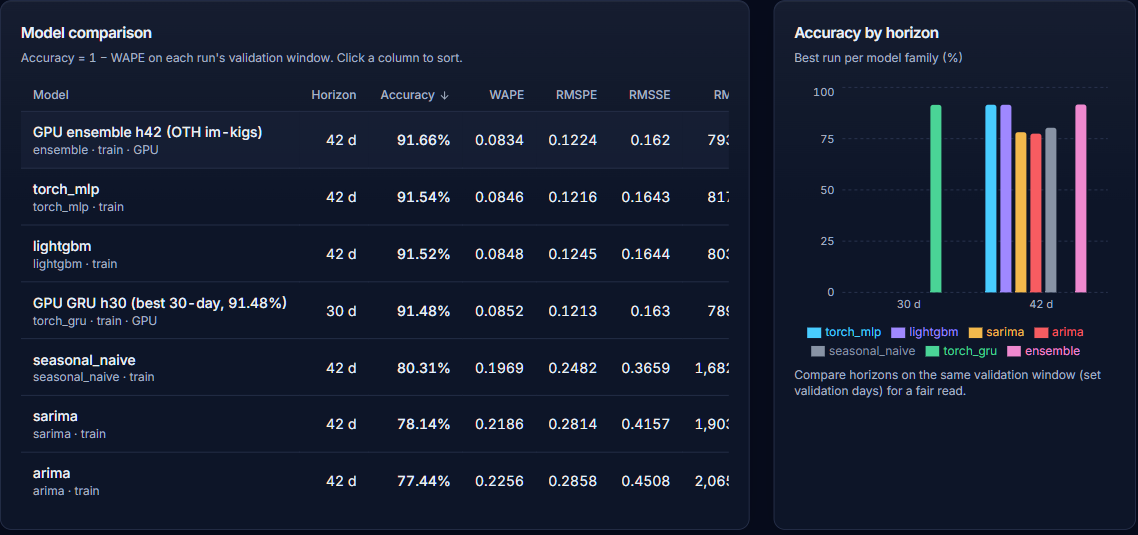
\includegraphics[width=0.49\textwidth]{figures/screens/model_lab_compare.png} \\
\footnotesize (a) Command Center: stores, latest forecast, latest plan & \footnotesize (b) Model Lab: leaderboard on one validation window \\[3pt]
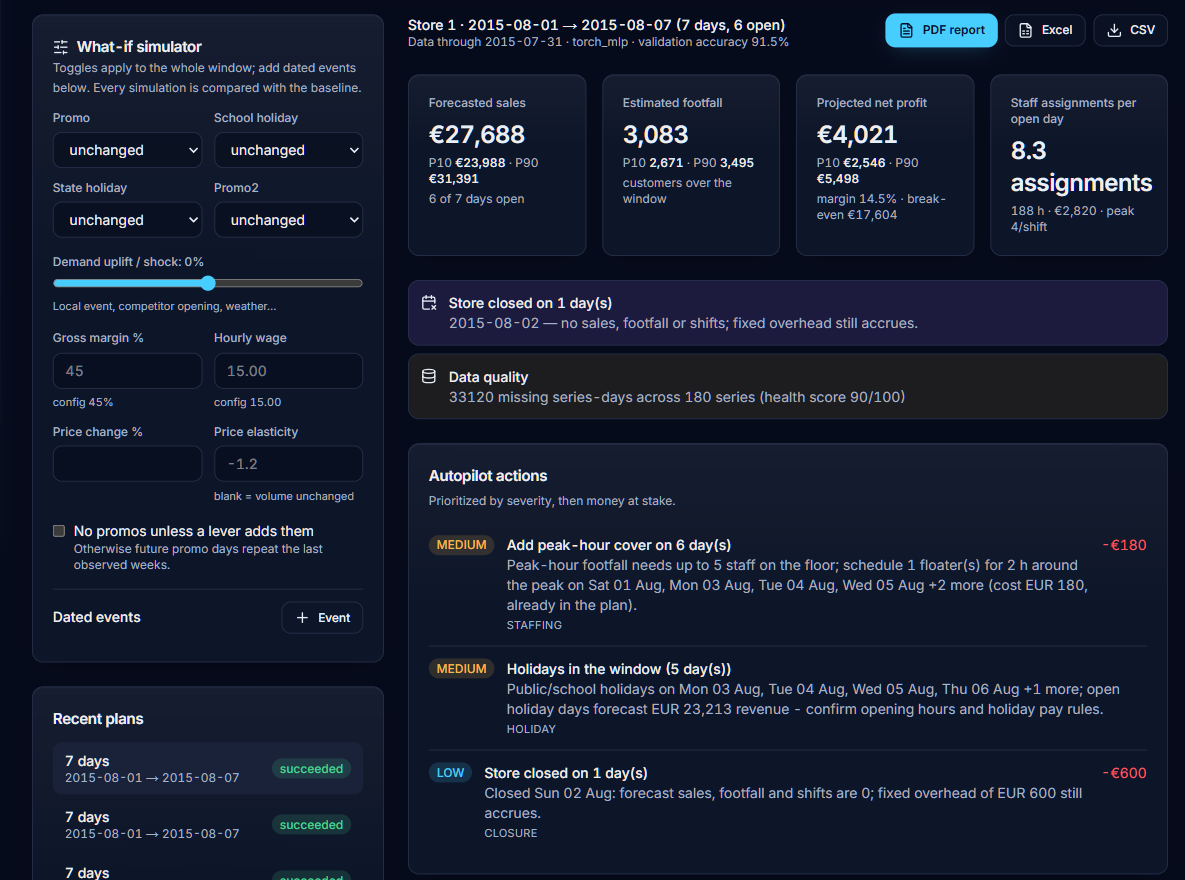
\includegraphics[width=0.49\textwidth]{figures/screens/autopilot_plan.png} &
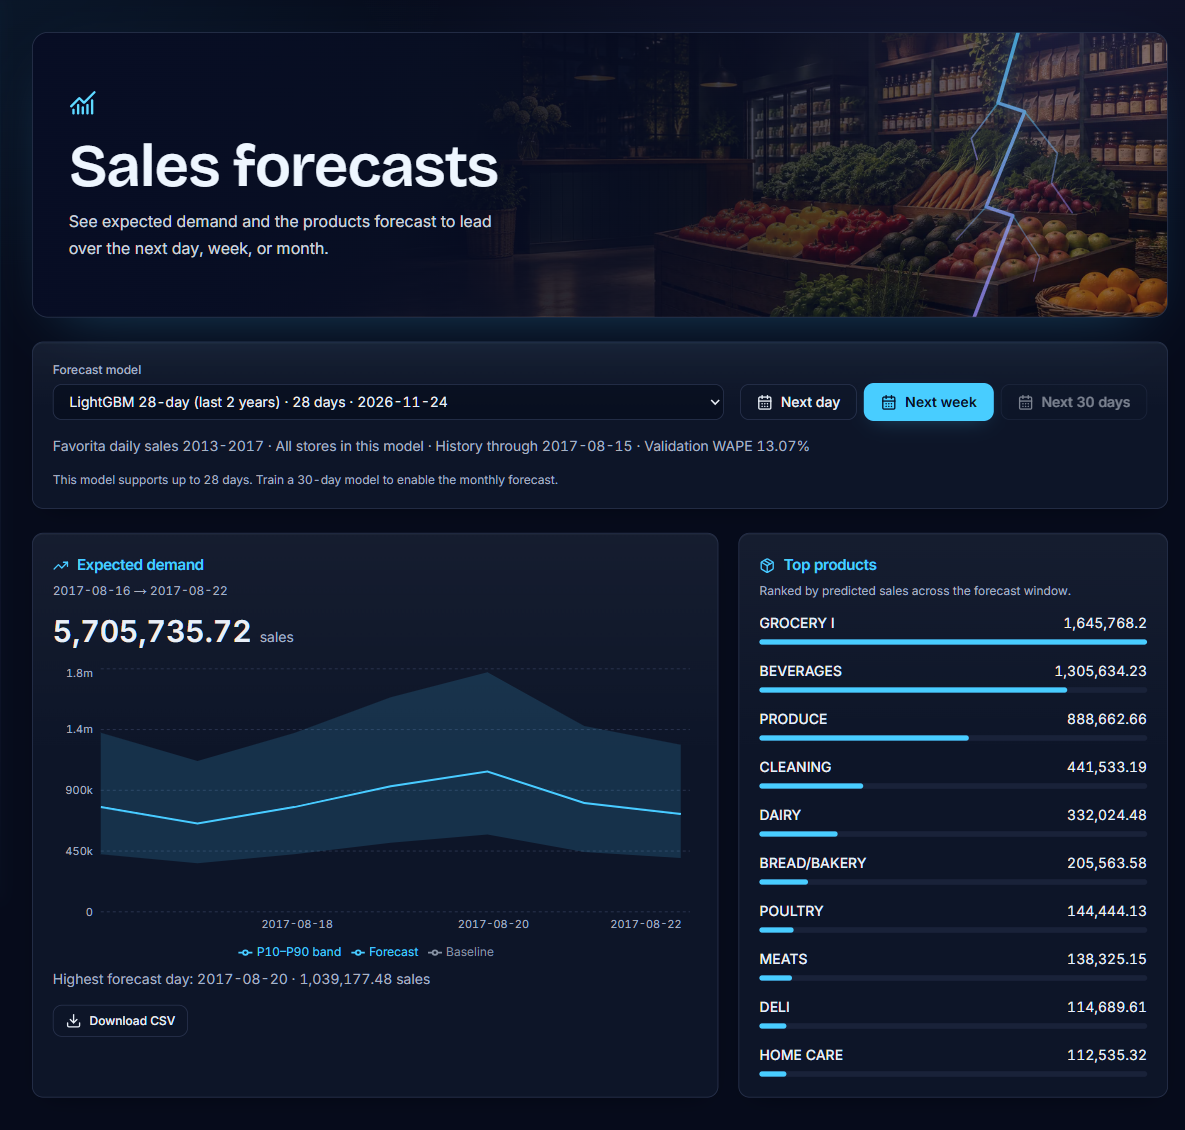
\includegraphics[width=0.49\textwidth]{figures/screens/favorita_forecast.png} \\
\footnotesize (c) Store Autopilot: KPI ranges, alerts, ranked actions & \footnotesize (d) Forecasts on Favorita: P10--P90 band and top product families \\
\end{tabular}
\caption{Screenshots of the running application with public demo data (Rossmann in a--c, Favorita
in d), captured at 1440$\times$900 on 24 Nov 2026 from commit \code{d3fadc8}. Account details are
hidden.}
\label{fig:screens}
\end{figure*}

\begin{figure}[t]
\centering
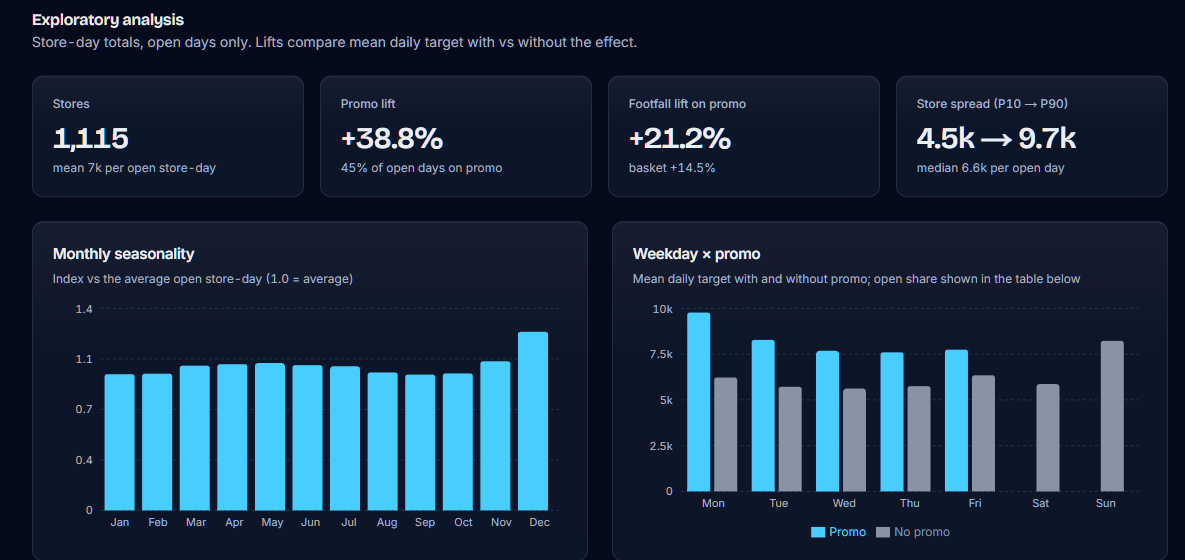
\includegraphics[width=\columnwidth]{figures/screens/eda_explore.png}
\caption{Exploratory analysis computed by the platform on Rossmann (open days): promotions lift mean
daily sales by 38.8\,\% and footfall by 21.2\,\%; December is the strongest month.}
\label{fig:eda}
\end{figure}

% =====================================================================================================
\section{Discussion}\label{sec:discussion}

\subsection{Answering the research question}
\textbf{H1 (supported).} With no test data used for model selection, LightGBM halves the
seasonal-naive WAPE at every one of eight origins (9.8 vs.\ 20.2\,\% on average; DM $p<10^{-4}$, sign
test $p=0.008$). This agrees with the M5 finding that global learned models beat per-series
statistical models on retail data~\cite{makridakis2022m5}. The size of the gap is consistent with
information the baseline cannot use (promotions, closures, holidays and cross-store patterns); that
attribution was not tested by ablation. The single split's 8.5\,\% is at the favourable end of the
year-round range (8.0--14.7\,\%).

\textbf{H2 (partly supported).} At 30 days the neural networks are significantly better than LightGBM
($-1.2$ points, $p<0.001$), and LightGBM is significantly better than SARIMA. At 42 days none of the
learned-model differences is significant over days: the ensemble's $-0.14$ points has $p=0.063$. The
store bootstrap would call it significant, but it treats days as fixed and so ignores shocks common to
all stores; for a decision about \emph{future} periods, the day-level DM test is the relevant one.

\textbf{H3 (not supported).} The integer program is not cheaper than the rules at equal
understaffing ($+0.00\,\%$ paid hours). The rules' rounding works as an implicit safety margin that
already lies on the optimiser's cost--service frontier. The optimisation model is still useful,
because it turns the safety margin into an explicit, priced choice (for example 3.4\,\% more hours for
32\,\% less understaffing).

\textbf{Uncertainty and operability.} The empirical bands of the learned models cover 77--84\,\% of
hold-out days, while ARIMA/SARIMA bands under-cover despite being more than twice as wide. Interactive
endpoints except the full EDA respond within 70\,ms, and the LightGBM result reproduces exactly across
machines.

\textbf{Answer to the RQ.} Yes for forecasting accuracy: the gain over the benchmark is large,
significant and stable across origins. No for cost savings from optimised staffing in the tested
setting, where the optimiser's contribution is to make the cost of service explicit.

\subsection{Trade-offs}
\textbf{Accuracy vs.\ cost.} The ensemble's 0.14-point gain over LightGBM at 42 days is not
significant, yet it requires training a GRU, which takes ten minutes on a laptop CPU without a GPU. LightGBM is the best default
when no GPU is available; the neural models pay off at the 30-day horizon. \textbf{Direct vs.\
recursive.} The direct strategy with a full-horizon lag offset avoids error accumulation and
leakage, but discards the most recent weeks of information for near-term days; a family of models
per lead-time bucket would recover it at higher training cost. \textbf{Rules vs.\ optimisation in
planning.} In the tested setting the integer program did not beat the rules at equal service
(\cref{sec:results-staffing}); its advantage is transparency about the cost of service. Richer roster
problems---part-time contracts, breaks, weekly hour limits, several days at once---are where
operations-research models usually outperform rules~\cite{ernst2004staff}.

\subsection{Limitations and threats to validity}
\begin{itemize}
\item \textbf{Model selection on the test window.} The single-split results (\cref{tab:accuracy})
  chose LightGBM's round count and the networks' best epoch on the reported window. The backtest uses
  an honest protocol, but only for LightGBM and the seasonal-naive model; the neural networks and the
  ensemble were not re-evaluated over rolling origins because each fit takes about ten minutes on the
  available CPU.
\item \textbf{Backtest scope.} Eight consecutive 28-day origins cover December 2014--July 2015, so
  the origins share most of their training data and are not independent; the confidence interval over
  origins is therefore approximate. 180 stores have no data for the second half of 2014.
\item \textbf{Staffing model.} The data are daily, so the hourly demand profile (30/45/25\,\% per
  shift, 14\,\% in the peak hour) is an assumption shared by the rules and the integer program.
  Footfall forecasts use a store-level average basket; the evaluation uses actual customer counts.
\item \textbf{Mixed environments.} 42-day ARIMA/SARIMA were trained in the local application rather
  than on the GPU host; data, stores and window are identical, but only WAPE and RMSSE were recorded
  for those two runs.
\item \textbf{Neural non-determinism.} MLP/GRU scores vary with device and batch size (8.46 vs.\
  8.72\,\% for the same MLP configuration); differences below about 0.3 percentage points between
  neural variants should not be over-interpreted.
\item \textbf{Data sets.} Rossmann is store-level and complete; Favorita was evaluated with one model.
  Item-level intermittent demand (M5) is supported but was not evaluated here.
\item \textbf{Planning parameters.} Costs, wages, basket sizes and shift shares are configured
  conventions---the Favorita and most Rossmann stores use demo values---so P\&L figures demonstrate
  mechanics, not real economics. The Autopilot was not validated against real staffing outcomes.
\item \textbf{Robustness.} The run-through found that neural models returned all-zero forecasts when
  a feature was constant in training (one-year history makes \code{lag\_364} empty); this was fixed
  by treating such inputs as uninformative and is now covered by a test. Similar edge cases may remain.
\item \textbf{Performance scope.} Latency was measured with a single client on loopback; concurrency,
  network latency and load were not tested.
\end{itemize}

% =====================================================================================================
\section{Future Work}\label{sec:future}
Each proposal addresses a limitation above. (1) Extend the honest rolling-origin backtest to the
neural networks and the ensemble on the GPU, and make honest early stopping the platform default
(model selection, backtest scope). (2) Evaluation on M5 item-level data with intermittent-demand
metrics and Tweedie/quantile objectives (data-set scope). (3) Conformal or quantile-head calibration
per horizon week to fix the narrow 30-day GRU band (uncertainty). (4) Probabilistic sequence
architectures such as DeepAR or TFT under the same protocol~\cite{salinas2020deepar,lim2021tft}
(model scope). (5) A multi-day roster model with contracts, breaks and weekly hour limits, solved
with the same integer-programming approach~\cite{ernst2004staff}, plus a field pilot with hourly
footfall data (staffing model). (6) Load tests with concurrent tenants and a hosted deployment that
follows the release checklist in \code{docs/PUBLIC\_PILOT.md} (performance scope).

% =====================================================================================================
\section{Conclusion}\label{sec:conclusion}
StorePulse AI shows that a complete forecasting-to-planning workflow can be built from open
components and evaluated with statistical discipline. Its contributions are a leakage-free direct
multi-horizon pipeline with a formal justification and an automated test, a model zoo compared on
identical windows, a rolling-origin backtest with honest model selection, significance tests that
separate real from apparent differences, and a staffing integer program benchmarked against rules
on realised demand. The evidence supports a large and stable accuracy gain of learned models over the
seasonal-naive benchmark (WAPE 9.8 vs.\ 20.2\,\% across eight origins), shows that small differences
between learned models are often not significant, and finds that optimised staffing does not save cost
over the rules in the tested setting but makes the cost of service explicit. Open questions concern
other data sets, honest backtests of the neural models and staffing with real hourly demand.

\section*{Use of AI Tools}
Claude Code (Anthropic) was used as an assistant throughout this project: for implementing and
debugging parts of the software, running and documenting the experiments, generating the charts,
and drafting the report and presentation text. All results were produced by the project's own code
and data, and I reviewed, verified and take responsibility for the final content.

\balance
\bibliographystyle{IEEEtran}
\bibliography{references}

% =====================================================================================================
\clearpage
\onecolumn
\appendices

\section{Reproducibility}\label{app:repro}
All commands run from the repository root on Windows PowerShell (adapt paths on Linux). Data files
are public downloads~\cite{kaggle2015rossmann,kaggle2021storesales} placed under
\code{data/raw/rossman dataset/} (not in the repository).

\begin{lstlisting}[language=bash]
# 1. Environment (Python 3.11+, Node 22)
cd backend
python -m venv .venv; .venv\Scripts\python -m pip install -e ".[dev,local]"
.venv\Scripts\python -m pip install torch            # optional, for MLP/GRU/ensemble

# 2. Tests (57 tests; the pipeline test needs data/raw/rossman dataset/train.csv)
.venv\Scripts\python -m pytest -q

# 3. Accuracy runs without database or queue (production code paths)
.venv\Scripts\python -m scripts.run_pipeline rossmann --families seasonal_naive lightgbm --horizon 42 --lgb-rounds 4000
.venv\Scripts\python -m scripts.run_pipeline rossmann --families seasonal_naive lightgbm --horizon 30 --lgb-rounds 4000

# 4. GPU runs as used for Table I (on a CUDA host; see docs/GPU_TRAINING.md)
python -m scripts.train_cli train --dataset rossmann --horizon 42 --families lightgbm torch_mlp torch_gru ensemble \
    --epochs 30 --lgb-rounds 4000 --lgb-param num_threads=16 --covariate-default Promo=0 --device cuda --run-name rossmann_h42_gpu
python -m scripts.train_cli train --dataset rossmann --horizon 30 --families lightgbm torch_mlp torch_gru ensemble sarima arima \
    --epochs 30 --lgb-rounds 4000 --lgb-param num_threads=16 --torch-param batch_size=2048 --covariate-default Promo=0 \
    --device cuda --run-name rossmann_h30_all

# 5. Full application, then the report's measurements and figures
.venv\Scripts\python -m scripts.local_stack up --present        # second terminal for the following
.venv\Scripts\python ..\report\scripts\collect_results.py         # report/data/*.csv
.venv\Scripts\python ..\report\scripts\backtest.py --origins 8 --horizon 28   # ~25 min, 4 cores
.venv\Scripts\python ..\report\scripts\significance.py            # DM tests, bootstrap
.venv\Scripts\python ..\report\scripts\staffing_ip.py --days 14   # integer program vs rules
.venv\Scripts\python ..\report\scripts\staffing_frontier.py       # cost-understaffing frontier
.venv\Scripts\python ..\report\scripts\bench_api.py --n 30        # API latency
.venv\Scripts\python ..\report\scripts\make_figures.py            # report/figures/*.pdf
.venv\Scripts\python ..\report\scripts\contrast.py                # WCAG contrast table
\end{lstlisting}

The run metadata of the GPU experiments (host, GPU, library versions, git commit, arguments) is
stored in \code{outputs/<run>/run.json}: the 42-day run used commit \code{adc082c} on 20 Nov 2026 and
the 30-day run commit \code{7854f31} on 23 Nov 2026, both with Python 3.11.16, PyTorch 2.14.1+cu126,
LightGBM 4.7.0 and pandas 3.1.1 on an NVIDIA RTX 6000 Ada.

\section{Test Scenarios}\label{app:tests}
\begin{center}
\small
\begin{tabular}{@{}p{0.2\textwidth}rp{0.68\textwidth}@{}}
\toprule
Module & Tests & What is verified \\
\midrule
\code{test\_api} & 7 & OpenAPI routes, error envelope for unauthenticated, invalid-token and validation errors, failed dispatch marks the job failed, product ranking, cancelled jobs are not restarted. \\
\code{test\_finance} & 5 & P\&L and workforce for sales, customers and units targets; minimum-staff floor; a sales target without average transaction value is rejected. \\
\code{test\_autopilot} & 14 & Window resolution, scenarios and baselines, closures, cold start, shift plans, action ranking, exports. \\
\code{test\_joins\_features} & 5 & Auxiliary joins at ingestion and forecast time, store features, calendar completion. \\
\code{test\_models\_metrics} & 14 & Metrics (RMSSE, $R^2$, pinball), \textbf{leakage scramble test}, intermittency and promo features, model round-trips, closed-day rule, ensembles, constant-input regression test. \\
\code{test\_eda} & 2 & EDA on Rossmann (seasonality, promotion and holiday lift); residual diagnostics by weekday and week ahead. \\
\code{test\_local\_stack} & 2 & Wi-Fi address selection skips VPN adapters; tunnel URL parsing. \\
\code{test\_pipeline} & 8 & End-to-end ingestion $\rightarrow$ features $\rightarrow$ training $\rightarrow$ forecast on Rossmann. \\
\midrule
Total & 57 & All passed in 38.5\,s on the laptop (\code{data/pytest\_results.xml}). \\
\bottomrule
\end{tabular}
\end{center}

Manual user-flow checks performed on the running application (24 Nov 2026): sign-in with empty
fields (blocked by validation), with a wrong password (error shown), and with valid demo credentials;
sign-out; creating 7- and 30-day forecasts; running a 7-day Autopilot plan; selecting a store and
loading its configuration; all eight pages at 375, 768 and 1024+ px width without horizontal
overflow; keyboard focus visible on navigation links.

\section{Supplementary Results}\label{app:supp}

\begin{table}[h]
\centering
\caption{Text contrast of the interface theme (WCAG~2.2 AA requires $\geq 4.5{:}1$ for normal text). Computed by \code{scripts/contrast.py}.}
\label{tab:contrast}
\small
\begin{tabular}{@{}lr@{}}
\toprule
Text / background pair & Contrast ratio \\
\midrule
Body text on card & 15.69 \\
Secondary text on card / page / muted fill & 8.46 / 9.12 / 7.38 \\
Primary button label & 10.25 \\
Accent (link) text on card & 9.86 \\
Inactive menu item & 8.74 \\
Warning / error / success text on card & 10.26 / 5.77 / 9.65 \\
\bottomrule
\end{tabular}
\end{table}

\begin{table}[h]
\centering
\caption{Data sets used (from the application's dataset records).}
\label{tab:datasets}
\small
\begin{tabular}{@{}lrrl@{}}
\toprule
Data set & Rows & Series & Date range \\
\midrule
Rossmann (all stores) & 1,017,209 & 1,115 & 2013-01-01 -- 2015-07-31 \\
Favorita store sales & 3,000,888 & 1,782 & 2013-01-01 -- 2017-08-15 \\
Synthetic demo & 1,095 & 3 & 2024-01-01 -- 2024-12-30 \\
\bottomrule
\end{tabular}
\end{table}

\begin{figure}[h]
\centering
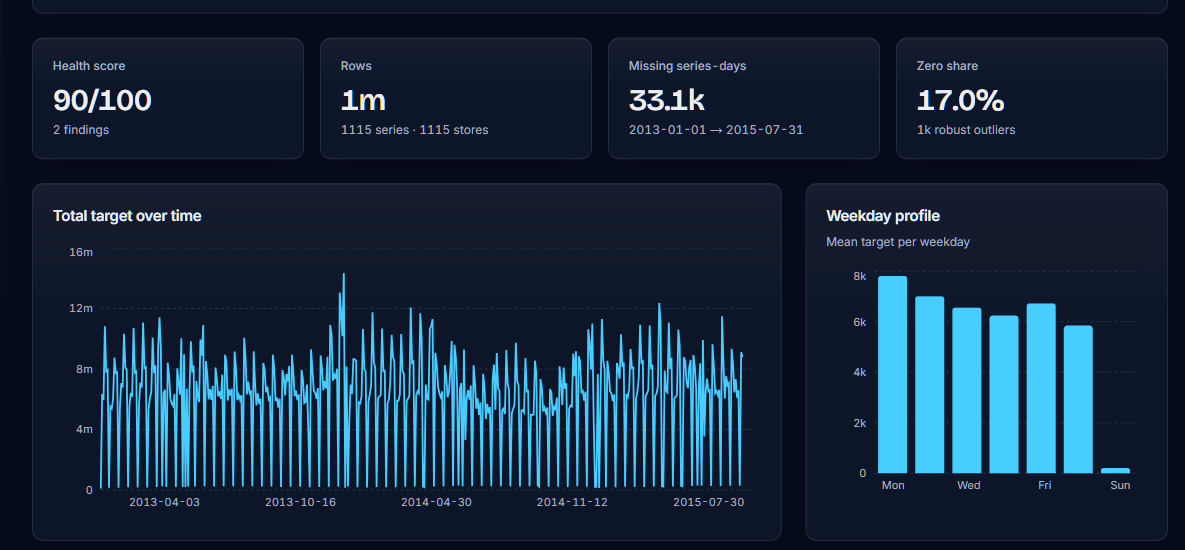
\includegraphics[width=0.78\textwidth]{figures/screens/eda_health.png}
\caption{Data-health view on Rossmann: health score 90/100, 33.1\,k missing series-days (the 180
stores with a six-month gap in 2014), 17.0\,\% zero days (closures) and a weekday profile with
very low Sunday sales.}
\label{fig:health}
\end{figure}

\begin{figure}[h]
\centering
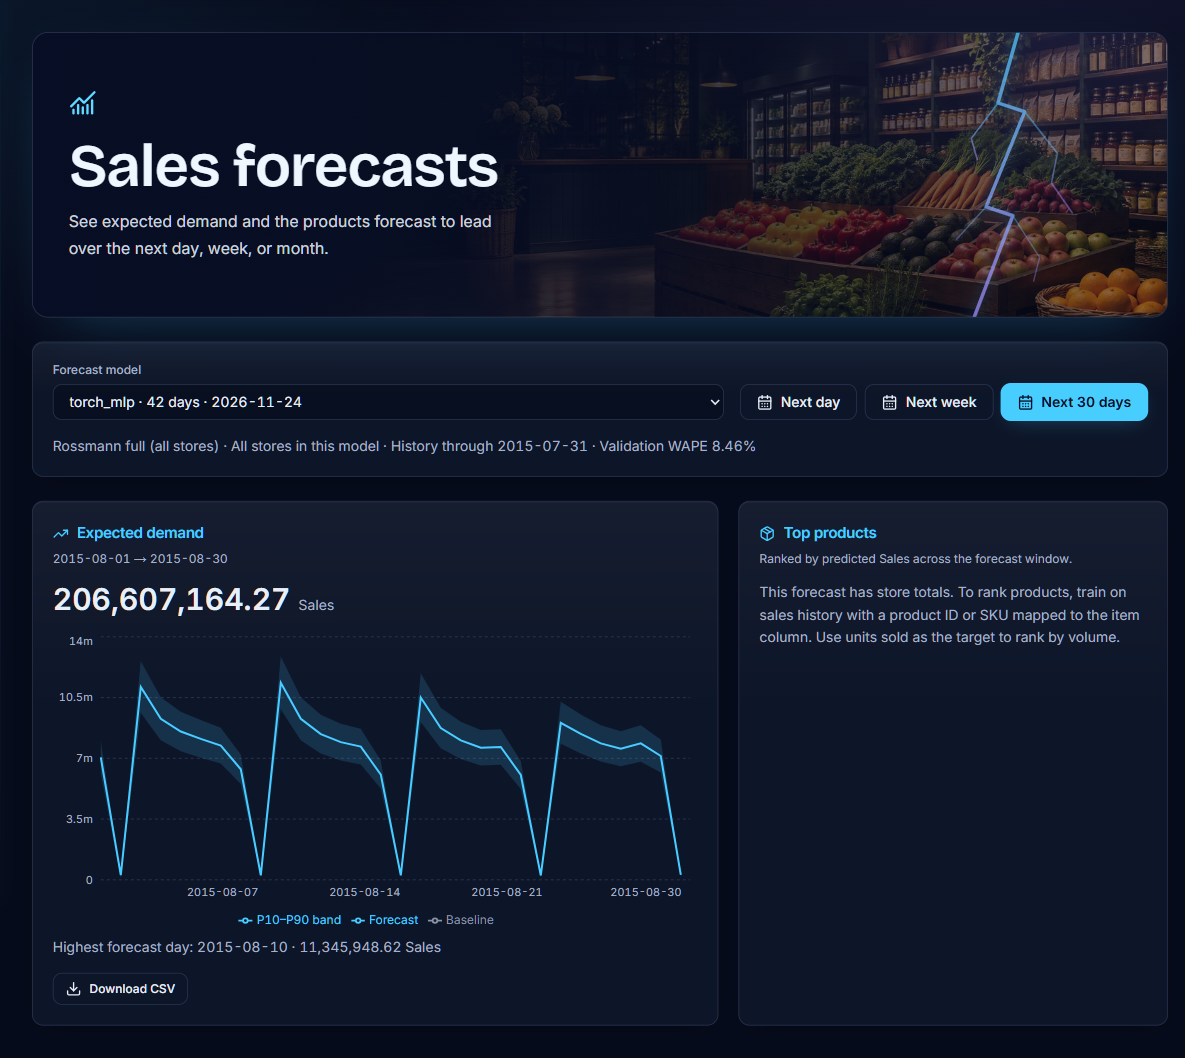
\includegraphics[width=0.6\textwidth]{figures/screens/forecasts.png}
\caption{Forecasts page: 30-day forecast for all Rossmann stores with the P10--P90 band (MLP model).}
\label{fig:forecastpage}
\end{figure}

\begin{figure}[h]
\centering
\begin{tabular}{cc}
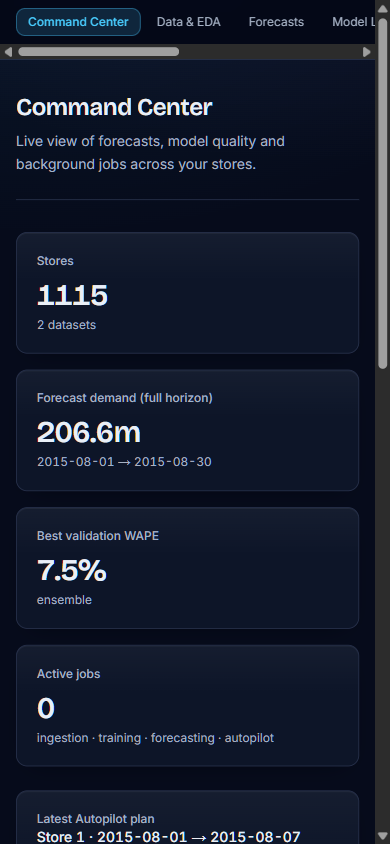
\includegraphics[height=8cm]{figures/screens/mobile_command_center.png} &
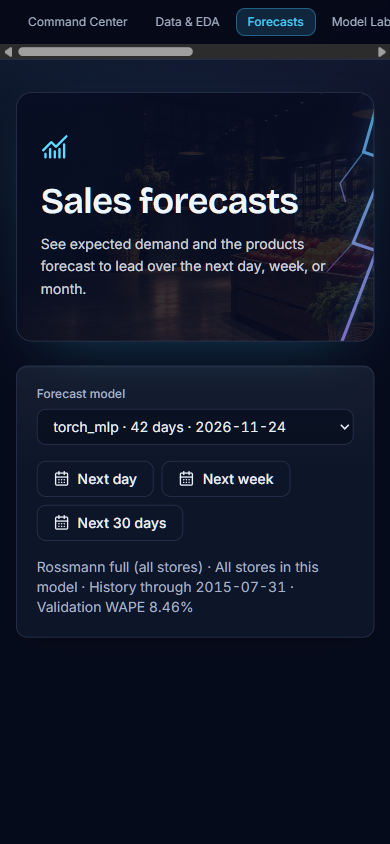
\includegraphics[height=8cm]{figures/screens/mobile_forecasts.png}
\end{tabular}
\caption{Phone layout (390$\times$844 px). Before a layout fix during the project, wide tables
widened the Model Lab page to 908 px on a 375 px screen; all pages now fit.}
\label{fig:mobile}
\end{figure}

\end{document}
